\chapter{Content of the CD}
Directories:
\begin{itemize}
  \item \textbf{src} - source code files
     \begin{itemize}
        \item \textbf{latex} - files required for building this document
        \item \textbf{dialog\_editor} - source files for the dialog editor
        \item \textbf{dialog\_editor\_vm} - virtual machine set up for launching the Dialog Editor
     \end{itemize}
  \item \textbf{pdf} - PDF version of the thesis
\end{itemize}

\chapter{Manual}

On the CD attached is a virtual machine image. It is located in the
{\tt dialog\_editor\_vm} directory, ready to be deployed using Virtual Machine
Manager.

\begin{enumerate}
  \item The first step is to create a NAT Virtual Network in Virtual Machine
        Manager. The manual on {\it libvirt} project wiki can be used\footnote{\url{http://wiki.libvirt.org/page/TaskNATSetupVirtManager}}.
  \item In Virtual Machine Manager select the button with label {\it Create a new virtual machine}.
  \item From options to install the operating system select the one with the label {\it Import existing disk image}.
  \item In the dialog select the virtual machine image from CD and choose memory and CPU settings. (give it at least 2048 MiB of RAM).
  \item In the final step, select the network you have created.
\end{enumerate}

After you create a new virtual machine, the machine should start
automatically.
Upon booting, you can login with default credentials
{\tt root} / {\tt smartvm}.
To start ManageIQ in your browser you will need an IP address of the
machine. The IP address can be found by running this command:

\begin{lstlisting}[language=bash]
$ ip a
\end{lstlisting}

The ManageIQ Self Service UI can be accessed
at {\tt http://[IP ADDRESS]/self\_service}.

\chapter{Figures}

  \begin{figure}[h]
    \centering
    \def\svgwidth{\columnwidth}
    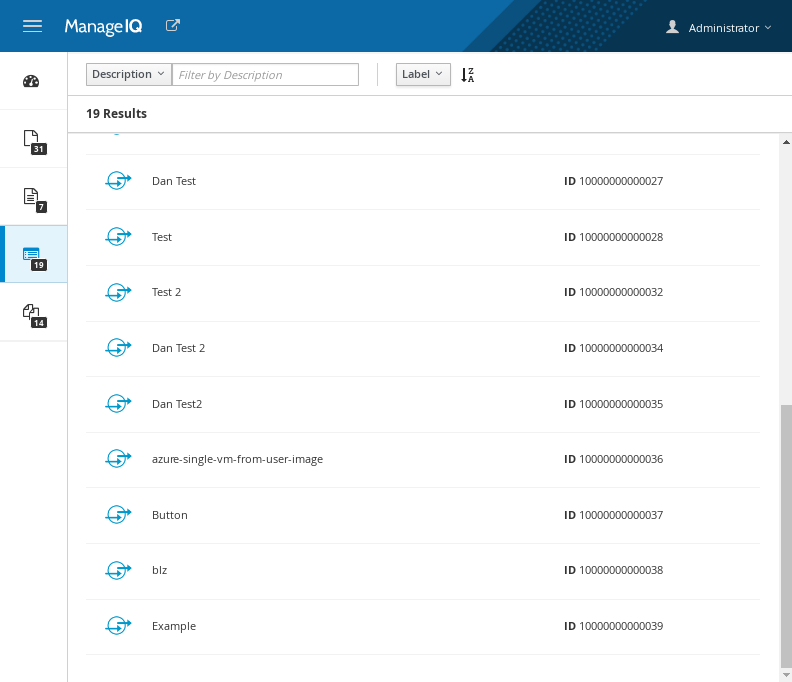
\includegraphics[width=15cm,keepaspectratio]{fig/dialog-list}
    \caption{List state for Dialogs in Self Service User Interface}
    \label{fig:dialog-list}
  \end{figure}

  \begin{figure}
    \centering
    \def\svgwidth{\columnwidth}
    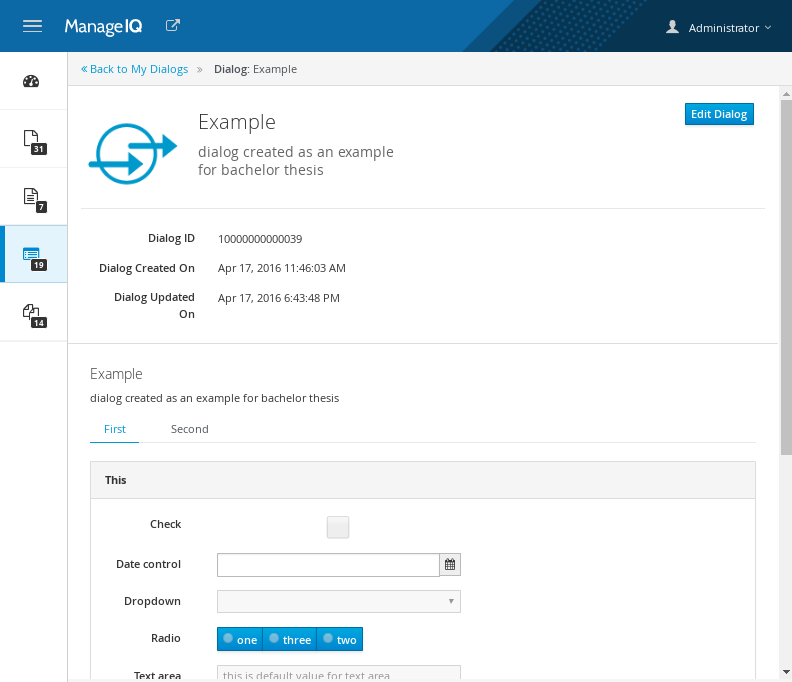
\includegraphics[width=15cm,keepaspectratio]{fig/dialog-detail}
    \caption{Detail state for Dialogs in Self Service User Interface}
    \label{fig:dialog-detail}
  \end{figure}

  \begin{figure}
    \centering
    \def\svgwidth{\columnwidth}
    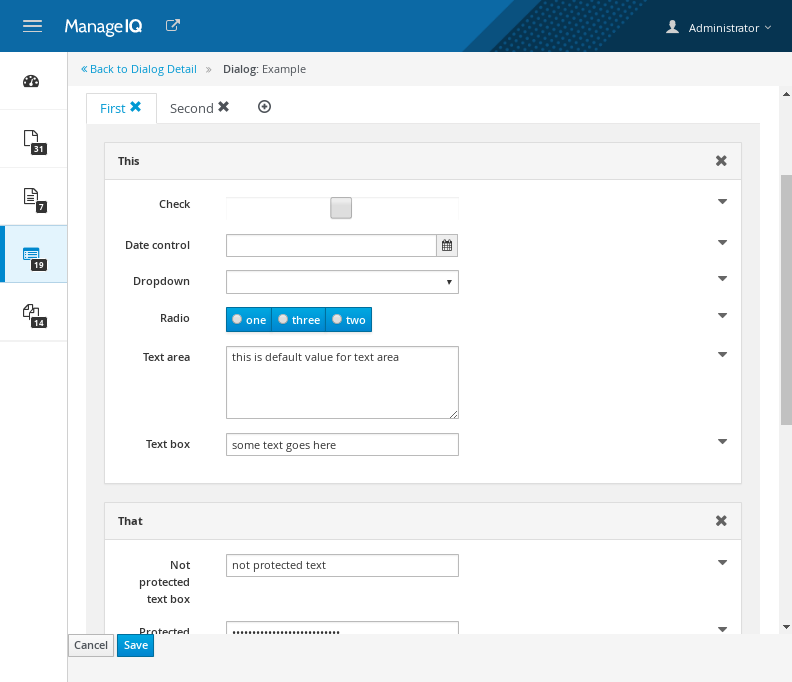
\includegraphics[width=13cm,keepaspectratio]{fig/dialog-edit}
    \caption{Example of Dialog in new Dialog Editor}\label{fig:dialog-edit}
  \end{figure}

  \begin{figure}
    \centering
    \def\svgwidth{\columnwidth}
    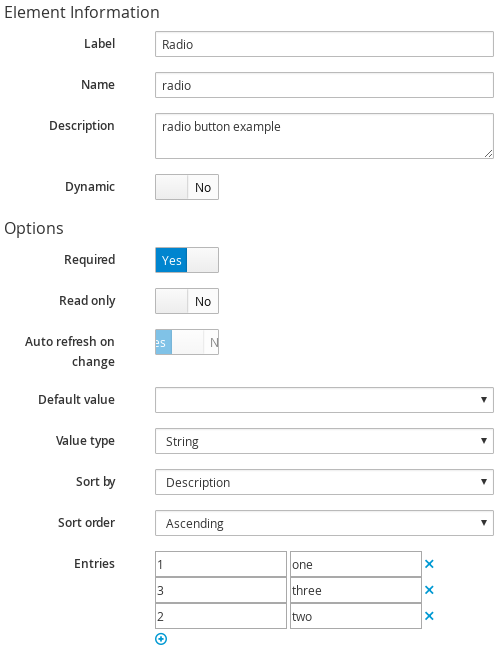
\includegraphics[width=12cm,keepaspectratio]{fig/dialog-modal}
    \caption{Modal for the Radio button field}\label{fig:dialog-modal}
  \end{figure}
